The goal of query optimization is to select the \textbf{best possible} strategy for query evaluation. \\

However the chosen plan is not always optimal.

\section{Query Trees and Heuristics for Query Optimization}

Optimizations techniques that apply \textbf{heuristics} to modify the internal representation of a query to \textbf{improve its performances}.\\

\textbf{Steps}:

\begin{itemize}
    \item Scanner and parser generate a data structure that corresponds to an \textbf{initial query representation}
    \item Query is optimized according to \textbf{heuristics} to obtain an optimized query representation
    \item \textbf{Query execution plan} is generated to execute groups of operations
\end{itemize}

One of the main \textbf{heuristics} is to apply \textbf{SELECT} and \textbf{PROJECT} before \textbf{JOIN} (because they reduce the size of the file before the join). Reduce the size of \textbf{intermediate results}.\\

\textbf{Data structures}:
\begin{itemize}
    \item {Query tree} (cfr. figure \ref{fig:tree}) used to represent a \textbf{relation algebra} expression
    \item \textbf{Query graph} (cfr. figure \ref{fig:graph}) is used for \textbf{relational calculus expression}
\end{itemize}

\begin{figure}[!h]
    \centering
    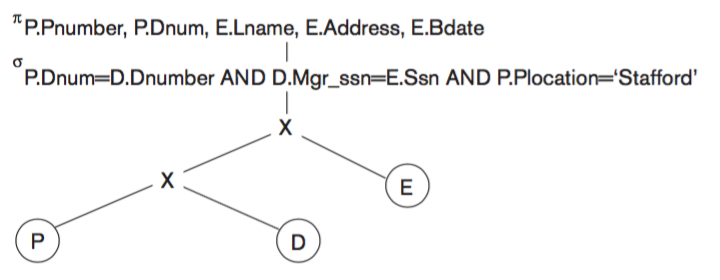
\includegraphics[scale=0.5]{chap19-1}
    \caption{Query tree}
    \label{fig:tree}
\end{figure}

\begin{figure}[!h]
    \centering
    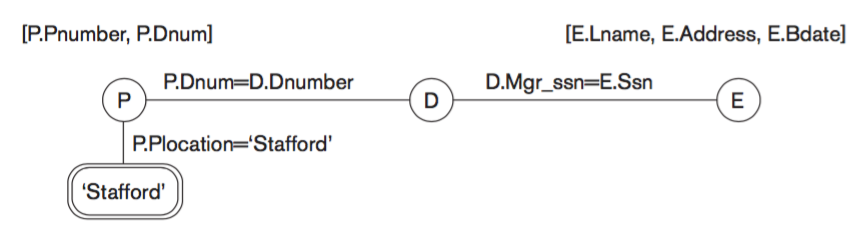
\includegraphics[scale=0.5]{chap19-2}
    \caption{Query graph}
    \label{fig:graph}
\end{figure}


\subsection{Notation for Query Trees and Query Graphs}

\textbf{Query tree} is composed of:

\begin{itemize}
    \item \textbf{Input relations} = leaves of the tree
    \item \textbf{Relational algebra operations} = internal nodes
\end{itemize}

\textbf{Execution} = execute an internal node whenever its operands are available.\\

\textbf{Query graph} is composed of:

\begin{itemize}
    \item \textbf{Input relations} = relations node (single circles)
    \item \textbf{Constant values} = constant nodes (double circles or ovals)
    \item \textbf{Selection and join conditions} = edges
\end{itemize}

\subsection{Heuristic Optimization of Query Trees}

Query parser first generates an initial query tree called \textbf{canonical query tree} but it might be very inefficient. So the \textbf{heuristic query optimizer} transforms it into a final query tree.\\

The optimizer includes rules of equivalence among relational algebra expression. \\

The list of the 16 transformation rules that can be applied can be found in the book at \textbf{page 698}. The most important ones are summarized below:\\

\begin{itemize}
    \item Cascade of SELECT and PROJECT
    \item Commutativity of SELECT, JOIN, UNION and INTERSECTION
    \item Associativity of JOIN, UNION and INTERSECTION
    \item Commuting PROJECT and RESTRICT
    \item Commuting RESTRICT and PROJECT
    \item Commuting RESTRICT and JOIN
    \item Commuting RESTRICT and SET Ops (UNION, INTERSECTION, MINUS)
    \item Commuting PROJECT and JOIN
    \item Commuting PROJECT and UNION
\end{itemize}

\textbf{Outline of a heuristic algebraic optimization algorithm}:
\begin{itemize}
    \item \textbf{Break up} any \textbf{SELECT} with conjunctive conditions into a cascade of SELECTS. It permits a greater degree of freedom in moving SELECT operations down the tree
    \item \textbf{Move} each \textbf{SELECT} as far down the tree as it is permitted by the attributes involved in the condition. If all the attributes are from the same table, move the SELECT to the leaf node for this relation. Otherwise move it where the corresponding tables are combined. 
    \item \textbf{Rearrange the leaf nodes}. Move the leaves with the most restrictive SELECT so they are executed first. Make sure that the ordering doesn't cause \textbf{Cartesian products}
    \item \textbf{Combine} cartesian product followed by a SELECT into a JOIN.
    \item \textbf{Move} the \textbf{PROJECT} as far as possible down the tree.
    \item \textbf{Identify} subgroups that can be executed by one algorithm
\end{itemize}

\textbf{Two approaches for evaluation}:

\begin{itemize}
    \item \textbf{materialized}: result of an operation is stored as a temporary result (physically materialized)
    \item \textbf{pipelined} (preferred): as resulting tuples are produced, they are forwarded directly to the next operation in the query sequence. 
\end{itemize}

